\chapter{Analisis dan Perancangan}
\label{chap:Analisis dan Perancangan}

Pada bab ini, penulis akan menjelaskan apa saja yang dilakukan dalam pengembangan \textit{Agglomerative Clustering} untuk Spark. Pengembangan dilakukan untuk mencapai tujuan yaitu mendapatkan pola dari dataset yang diolah. Pola yang ingin didapatkan meliputi perhitungan rata-rata, nilai maksimum, nilai minimum dan nilai standar deviasi dari setiap attribut yang ada pada data. Selain itu, perlu didapatkan juga jumlah anggota pada setiap \textit{cluster} yang dihasilkan dari algoritma \textit{Agglomerative Hierarchical Clustering}.


\section{Analisis Perangkat Lunak}

asdasd

\section{Perancangan Perangkat Lunak}

Pada bagian ini, akan dijelaskan perancangan perangkat lunak.  Perancangan termasuk diagram \textit{use case}, skenario, diagram kelas, dan rancangan antarmuka. 

\subsection{Diagram Use Case dan Skenario}

Diagram \textit{use case} merupakan sebuah pemodelan untuk perilaku dari perangkat lunak yang akan dibuat. Diagram \textit{use case} digunakan untuk mengetahui fungsi apa saja yang ada dalam perangkat lunak. Fungsi-fungsi dari perangkat lunak akan dioperasikan oleh satu pengguna. Cara kerja dan perilaku dari perangkat lunak akan dijelaskan dalam bentuk diagram \textit{use case}. Diagram \textit{use case} dapat dilihat pada Gambar ~\ref{fig:usecase}.

\begin{figure}[H]
    \centering  
    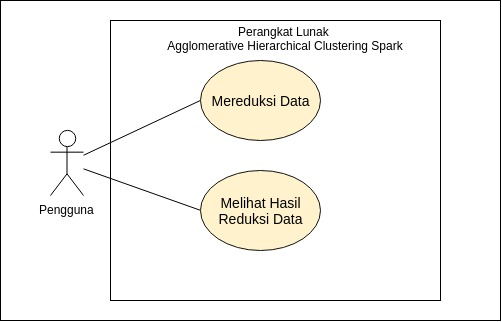
\includegraphics[scale=0.7]{usecase}  
    \caption[Gambar diagram \textit{use case} perangkat lunak \textit{Agglomerative Hierarchical Clustering}]{Gambar diagram \textit{use case} perangkat lunak \textit{Agglomerative Hierarchical Clustering}} 
    \label{fig:usecase} 
\end{figure}

Bedasarkan gambar diagram \textit{use case} diatas, berikut adalah skenario yang ada:

\begin{enumerate}

\item Nama \textit{use case}: Mereduksi data

\begin{itemize}
\item Aktor: Pengguna

\item Pre-kondisi: data yang akan diolah dimasukan kepada HDFS

\item Pra -kondisi: hasil reduksi disimpan pada HDFS

\item Deskripsi: Fitur untuk menjalankan program untuk mereduksi data

\item Langkah-langkah:

\begin{enumerate}

\item Pengguna mengisi JAR \textit{path}, \textit{input path}, dan \textit{output path}

\item Pengguna mengisi jumlah \textit{executor} dan besar \textit{executor memory}

\item Pengguna mengisi jumlah partisi, batas maksimum objek, tipe metode, dan \textit{cut-off distance} 

\item Pengguna menekan tombol \textit{submit}

\item Sitem melakukan pengolahan data dengan algoritma \textit{Agglomerative Hierarchical Clustering} pada \textit{cluster} Hadoop

\item Sistem membuka tab baru untuk melihat tahap dan progres program

\item Sistem menyimpan hasil reduksi pada HDFS
\end{enumerate}

\end{itemize}


\item Nama \textit{use case}: Melihat data

\begin{itemize}
\item Aktor: Pengguna

\item Pre-kondisi: data yang akan ditampilkan sudah disimpan pada HDFS

\item Pra -kondisi: menampilkan data yang ada pada HDFS

\item Deskripsi: fitur untuk melihat data hasil reduksi

\item Langkah-langkah:

\begin{enumerate}

\item Pengguna mengisi \textit{path} dimana data disimpan pada HDFS

\item Sistem menampilkan data-data pada direktori tersebut

\end{enumerate}

\end{itemize}

\end{enumerate}


\subsection{Diagram Kelas}

\subsection{Rancangan Antarmuka}